\todo[inline]{Introductory words}

As already described in Chapter \ref{sec: Wetting_SurfaceTension}, there are various ways to describe the interface. Hydrodynamic models describe the interface such that the material values jump at the phase transition. On the other hand, a diffuse interface describes the quantities differently. \todo{picture of interfaces}

\section{Phase Field Method in the Spirit of Cahn and Hillard}
The phase field method traces back to the idea of van der Waals \cite{vanderwaals1979ThermodynamicTheoryCapillarity}, who described the interface between two immiscible fluids from a thermodynamic perspective. In this description, the material properties transition continuously within a thin layer. Both phases exist within this layer (see grey area in figure \ref{fig: DiffusiveInterface}).
\begin{figure}[h]
    \centering
    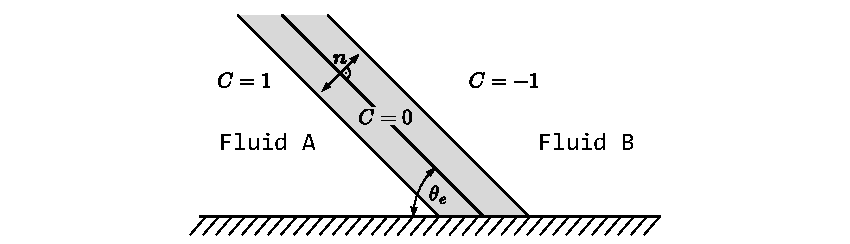
\includegraphics[width=.95\textwidth]{Pictures/DiffusiveInterface.pdf}
    \caption{Diffusive Interface for a binary fluid system. }
    \label{fig: DiffusiveInterface}
\end{figure}


Building on this, Cahn and Hillard \cite{johnw.FreeEnergyNonuniform1958} derived a description of the free energy in a volume with unequal composition as a function of an order parameter $C$ for time-dependent problems. In closed form, it reads:
\begin{equation}
\label{eq: CahnHillard}
    \partial C + \textbf{u} \cdot \nabla C = \nabla \cdot \left(\kappa \nabla \phi(C)\right).
\end{equation}
Here, $\textbf{u}$ is the velocity, $\kappa$ is a diffusion coefficient, often called mobility, and $\phi$ is a chemical potential. The order parameter indicates which phase is present and ranges between $-1$ and $1$ for a two-phase system. Mobility can be related to the Péclet number, which represents the ratio of advective to diffusive flows with a characteristic path length ($L_{char}$), velocity ($u_{char}$), and a characteristic chemical potential\cite{cai2015NumericalSimulationWetting, holzinger2021DirectNumericalSimulation}.

The chemical potential is defined as the derivative of the free energy with respect to the order parameter. In the system under consideration, the total free energy consists of the mixing energy and the interfacial density energy. According to \cite{yue2010SharpinterfaceLimitCahn}, the system's free energy is influenced by two factors; defined over the volume $\Omega$ and the surface $\partial\Omega$ \todo{check!!!}
\begin{equation}
    F(C, \nabla C) = \int_{\Omega} f_{mix} (C, \nabla C) d\textbf{x}+ \int_{\partial\Omega}f_w(C) dS
\end{equation}
The first integral represents the mixing energy density $f_{mix}$, and the second represents the wall $f_w$.
\subsection{Mixing Energy}
Cahn and Hillard defined a mixing energy that depends on the order parameter and its gradient:
\begin{equation}
    F_{mix}(C, \nabla C) = \int_{\Omega} f_{mix} (C, \nabla C) d\textbf{x} = \int_{\Omega}\left(\frac{\lambda}{\epsilon^2}\Psi(C)+\frac{\lambda}{2}\vert\nabla C\vert^2\right)d\textbf{x}
\end{equation}\todo{check if right function}
The integral consists of two terms. The first term separates the phases from each other, while the second term mixes the phases. $\lambda$ is a mixing energy parameter, $\epsilon$ is a measure of the thickness of the interface\todo{check if already mentioned}, and $\Psi$ is a potential. The potential is chosen according to Ginzburg and Landau\todo{cite} such that it has two minima at positions $-1$ and $1$, and is given by
\begin{equation}
    \Psi(C)= \frac{1}{4}\left(C^2-1\right)^2.
\end{equation}
From this, the following representation for the chemical potential arises:
\begin{equation}
    \label{eq: chempotentialMIXING_pahseFieldMethod}
     \Phi(C):= \frac{\partial F(C)}{\partial \chi} = \frac{\lambda}{\epsilon^2}\Psi'(C)-\lambda\nabla^2C.
\end{equation}
In the case of a planar interface and in equilibrium, the order parameter normal to the interface can be described by
\begin{equation}
    C(n) = \tanh\left(\frac{n}{\sqrt{2}\epsilon}\right)
\end{equation}\cite{cai2015NumericalSimulationWetting}. Here, $n$ is the normal to the interface. In equilibrium, the thickness of the diffuse interface remains constant, and approximately $90\%$ of the changes in $C$ occur over a range of $L=4.1641\epsilon$. Also, in the case of equilibrium, the surface tension equals the integral of the free energy density at the interface, from which a description for the surface tension can be derived. \todo{src, jaqcmin2000?}
\begin{equation}
\label{eq: surfacetensionEqui}
    \sigma = \int_{-\infty}^{\infty}\lambda\left( \frac{d\varphi}{dn}  \right)^{2}= \frac{2\sqrt{2}}{3} \frac{\lambda}{\epsilon}
\end{equation}
\subsection{Wall Energy}
Jaqcmin \cite{jacqmin1999CalculationTwoPhaseNavier} postulated a wall energy of the form
\begin{equation}
    F_w=\int \sigma g(C)dA, 
\end{equation}
whereby the wall energy is solely a function dependent on the fluid composition directly at the wall. From this, a function for the wall energy density can be derived \cite{jacqmin2000ContactlineDynamicsDiffuse}.
\begin{equation}
    f_w(C)=-\sigma \cos\theta_e \frac{C(3-C^2)}{4} + \frac{\sigma_{S_L}+ \sigma_{S_V}}{2}
\end{equation}
When only one of the phases is present, this equation only returns the respective surface tension. However, Yue et al. \cite{yue2011CanDiffuseinterfaceModels}\todo{check if right paper} pointed out that this description of wall energy for equilibrium contact angles close to $0°$ or $180°$ is difficult to reproduce and the model is not capable of handling precursor films. 

\section{Navier Stokes and Cahn Hillard Equations}\todo{new title}

The Navier Stokes and Cahn-Hillard equations are:
\begin{align}
    \nabla \cdot \textbf{u} &= 0 \\
    \rho\bigg(\frac{\partial\textbf{u}}{\partial t}+\textbf{u}\cdot\nabla\textbf{u}\bigg)&=-\nabla p+\mu\Delta\boldsymbol{u}+\phi\nabla C\\
    \frac{\partial C}{\partial t}+\textbf{u}\cdot\nabla C&=\nabla\cdot(\kappa\nabla G).
\end{align}
Herein, $G$, the chemical potential in the bulk, as well as the chemical potential of the surface $L$, and a body force $B$ were determined via a variational procedure \cite{jacqmin2000ContactlineDynamicsDiffuse}\todo{cite quian2006}. They are defined as follows:
\begin{align}
    \phi&=\lambda\Bigg[-\nabla^{2}C + (C^2-1)\frac{C}{\epsilon^2}\Bigg]\\
    L&= \lambda \textbf{u}\cdot \nabla C+ f'_w(C)\\
    \boldsymbol{B} &= \phi\nabla C
\end{align}
The boundary conditions on the solid substrate are:
\begin{align}
\textbf{v} &= \textbf{v}_w,\\
\textbf{n}\cdot \nabla \phi &= 0, \\
\frac{\partial C}{\partial t}+\textbf{v}\cdot\nabla C&=-\Gamma L,
\end{align}
Herein, $\boldsymbol{v}_w$ is the velocity of the wall, with $\boldsymbol{v}_w = 0$. The adhesion condition implies that the movement at the wall only occurs through the Cahn-Hillard diffusion \cite{yue2011WallEnergyRelaxation}. The second boundary condition defines that no flow is allowed through the wall. The third boundary condition allows for a relaxation of the wall layer driven by the surface potential $L$ with $\Gamma$ as a constant, which is
